% This LaTeX document needs to be compiled with XeLaTeX.
\documentclass[a4paper]{article}
\usepackage[utf8]{inputenc}
\usepackage{amsmath}
\usepackage{amsfonts}
\usepackage{amssymb}
\usepackage[version=4]{mhchem}
\usepackage{stmaryrd}
\usepackage{graphicx}
\usepackage[export]{adjustbox}
\graphicspath{{./images/}{../cose da aggiungere/pittogrammi/}{../cose da aggiungere/privacy_conformita/}}
\usepackage{caption}
\usepackage[fallback]{xeCJK}
\usepackage{polyglossia}
\setmainlanguage{italian}

\usepackage{float}
\usepackage{tabularx}

\usepackage{titling}
\pretitle{\begin{center}
\includegraphics[width=\textwidth]{images/WATT+}\\[6em]}
\posttitle{\end{center}}

\usepackage{fontspec}

%\IfFontExistsTF{Noto Serif CJK JP}
%{\setCJKmainfont{Noto Serif CJK JP}}
%{\IfFontExistsTF{STSong}
%  {\setCJKmainfont{STSong}}
%  {\IfFontExistsTF{Droid Sans Fallback}
%    {\setCJKmainfont{Droid Sans Fallback}}
%    {\setCJKmainfont{SimSun}}
%}}
%
%\setmainlanguage{italian}
%\IfFontExistsTF{CMU Serif}
%{\setmainfont{CMU Serif}}
%{\IfFontExistsTF{DejaVu Sans}
%  {\setmainfont{DejaVu Sans}}
%  {\setmainfont{Georgia}}
%}


\title{\Huge ROLLERSHAPE+}   
\date{}

\begin{document}

\maketitle

\captionsetup{singlelinecheck=false}
%
\noindent Leggere attentamente il manuale di istruzioni e seguire le istruzioni prima dell'uso.

\newpage

\tableofcontents

\newpage

\section{Prefazione}
Gentile utente: 

Vi invitiamo a scegliere il prodotto più recente della nostra azienda, la macchina di rulli a sfere interni, che utilizzano un'innovativa tecnologia di microvibrazione compressione. Questa tecnologia è ottenuta attraverso una maniglia cilindrica intelligente che Ruota di $360^{\circ}$. Per la rotazione si utilizza un rullo con 50 sfere in silicone sul manico più grande. Cura del corpo; un altro rullo con 60 palline di silicone su un manico più piccolo Viene utilizzato per la cura del viso e del collo. Le sfere di silicone vengono inserite in forma a nido d'ape con densità e diametro specifici. La direzione di rotazione e la pressione assicura che la microcompressione venga trasmessa al tessuto. L'impugnatura unica Produce una compressione meccanica e microvibrazioni sulla pelle, che non possono essere replicate. con le mani o con altre tecniche. La "terapia microvibrazionale compressiva" sostituisce... il metodo tradizionale di "aspirazione massaggio di trazione", utilizzando la microcompressione invece della suzione e la microvibrazione invece di trazione. Applicato al corpo, aiuta a migliorare il drenaggio linfatico e circolazione e miglioramento della circolazione profonda. Disintossicazione. sollievo muscolare

rigidità e Dolore, scomporre i depositi di grasso sottocutaneo,\\
Elimina la cellulite, riduce la cellulite e modella la tua figura. Già dopo pochi utilizzi. Con questi trattamenti il tuo corpo ridurrà immediatamente il suo volume di 1 o 2 taglie! Applicato Sul viso, aiuta a migliorare la formazione dei vasi sanguigni, favorendo così produzione di collagene ed elastina, aumentando l'apporto di ossigeno, nutrendo e Illumina i tessuti dall'interno. Rilassa e regola i muscoli e aiuta per ridurre le linee di espressione.

Migliora l'aspetto, riduce il gonfiore, combatte il rilassamento cutaneo e ringiovanisce la pelle. affrontare in modo significativo. La terapia microvibrazionale compressiva è appositamente progettato per il ringiovanimento cutaneo non invasivo, il Rimodellamento corporeo e fisioterapia. È l'ultima generazione in fatto di cura Rimodellamento del corpo per viso, collo, spalle, braccia, petto, schiena, vita, addome, glutei, gambe e piedi, tra gli altri. Terapia microvibrazionale di La compressione è un trattamento che può riattivare la circolazione sanguigna e un metodo che può trattare patologie complesse come la stasi linfatica, linfedema e cellulite, migliorando così la nutrizione e l'ossigenazione della pelle Cellulare. La terapia microvibrazionale compressiva è un'innovativa combinazione di bellezza e salute.

\section{Simboli}
\begin{figure}[H]
	\centering
	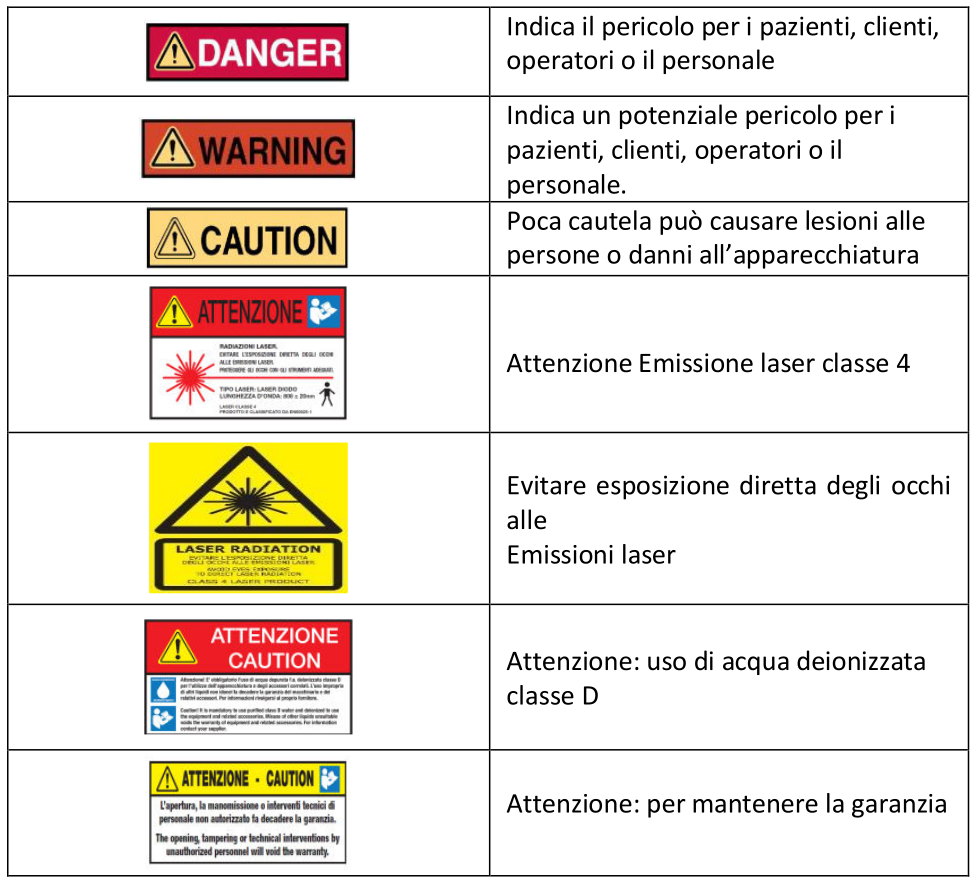
\includegraphics[width=\linewidth]{pittogrammi_1}
%	\caption{}
	\label{fig:pittogrammi1}
\end{figure}
\begin{figure}[H]
	\centering
	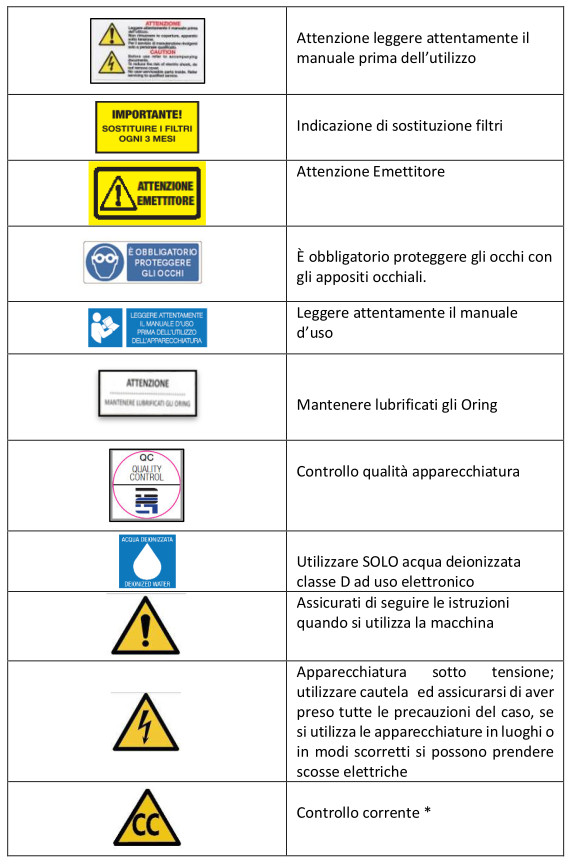
\includegraphics[width=\linewidth]{pittogrammi_2}
%	\caption{}
	\label{fig:pittogrammi2}
\end{figure}
\begin{figure}[H]
	\centering
	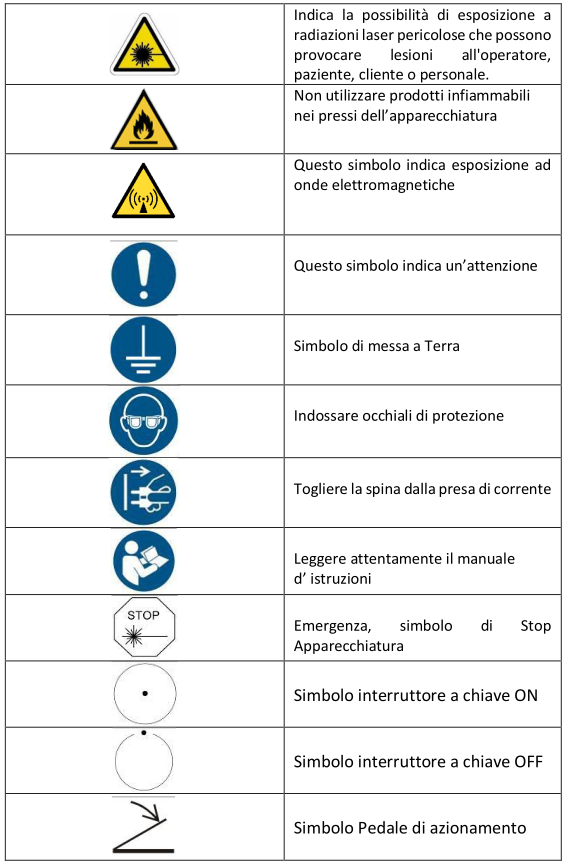
\includegraphics[width=\linewidth]{pittogrammi_3}
%	\caption{}
	\label{fig:pittogrammi3}
\end{figure}
\begin{figure}[H]
	\centering
	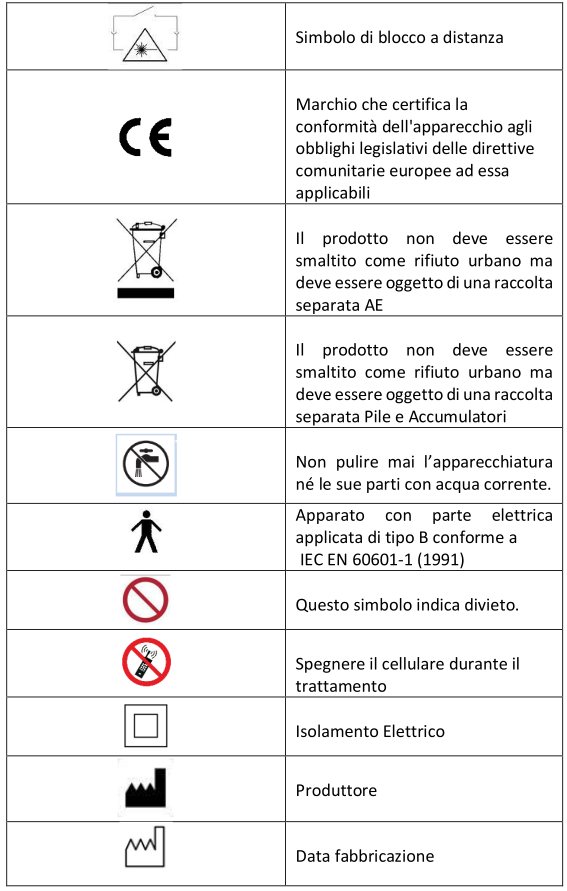
\includegraphics[width=\linewidth]{pittogrammi_4}
%	\caption{}
	\label{fig:pittogrammi4}
\end{figure}
\begin{figure}[H]
	\centering
	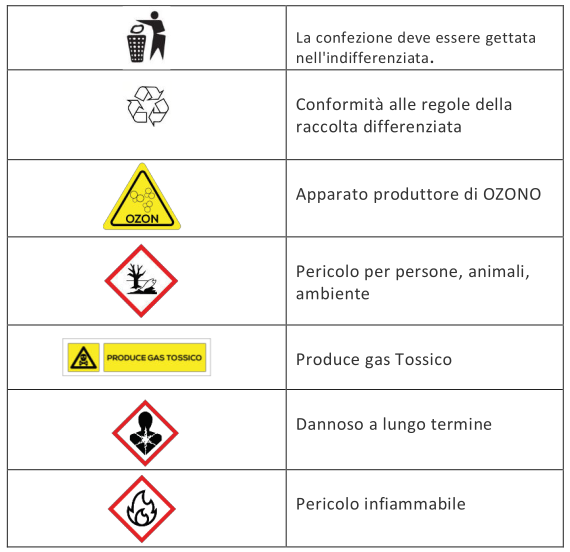
\includegraphics[width=\linewidth]{pittogrammi_5}
%	\caption{}
	\label{fig:pittogrammi5}
\end{figure}


\section{Introduzione dei principi}
Il dispositivo a rulli interni è un trattamento non invasivo di Microvibrazione tramite compressione meccanica. Il principio è che la sfera in silicone Ruota di $360^{\circ}$ lungo il rullo per generare microvibrazioni di compressione. Ruotando e applicando pressione sulla pelle si produce un effetto di "compressione". pulsante", con un movimento alternato, continuo di impastamento e spinta trazione. Il tessuto subisce pressione e sollevamento, senza comprimere o danneggiare il pelle. La pressione esercitata sul tessuto allunga le cellule e le stimola. attività cellulare naturale e profonda, flusso sanguigno e ossigenazione. I depositi di grasso vengono pressurizzati e allentati per la decomposizione, riduce ed elimina la cellulite. Inoltre, esercita pressione sui gruppi muscolari. muscoli profondi per ammorbidirli e allungarli completamente, riducendo riducendo così la rigidità e il dolore muscolare e accelerando il metabolismo.

Elimina la stagnazione e l'accumulo di liquidi, condiziona i tessuti e Rassoda la pelle, rimodellando il corpo. Stimola anche i fibroblasti. Aumenta la produzione di collagene ed elastina, aumenta il flusso sanguigno e L'ossigeno aumenta. Di conseguenza, le rughe vengono levigate e il Riduce il gonfiore e le borse sotto gli occhi e la pelle risulta ringiovanita e rassodata. Questa tecnologia è clinicamente provata per tonificare i muscoli e scolpire il corpo e il viso per ringiovanire, oltre ad aiutare a ridisegnare e rassodare il seno.

\begin{figure}[H]
\begin{center}
  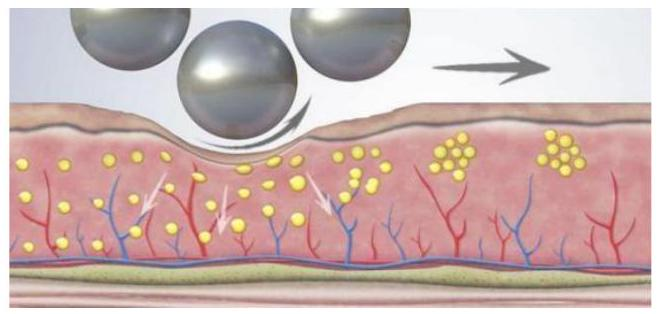
\includegraphics[alt={},max width=\textwidth]{31d8a32b-88de-483b-82f7-0d2b231ca911-04_314_659_1146_196}
\captionsetup{labelformat=empty}
\caption{Rimodellamento dell'azione}
\end{center}
\end{figure}

Rimodella i contorni e leviga le rughe.

\begin{figure}[H]
\begin{center}
  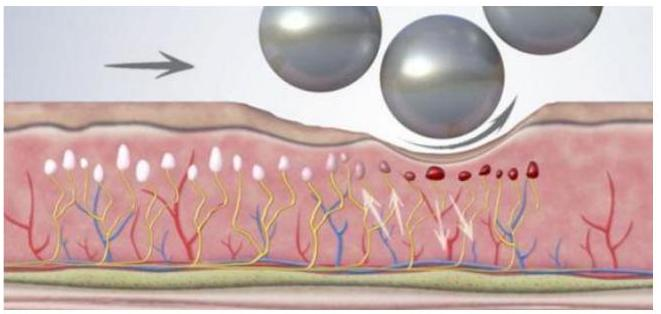
\includegraphics[alt={},max width=\textwidth]{31d8a32b-88de-483b-82f7-0d2b231ca911-04_314_661_1790_173}
\captionsetup{labelformat=empty}
\caption{Sedazione}
\end{center}
\end{figure}

Migliora l'ossigenazione ed elimina il dolore.\\
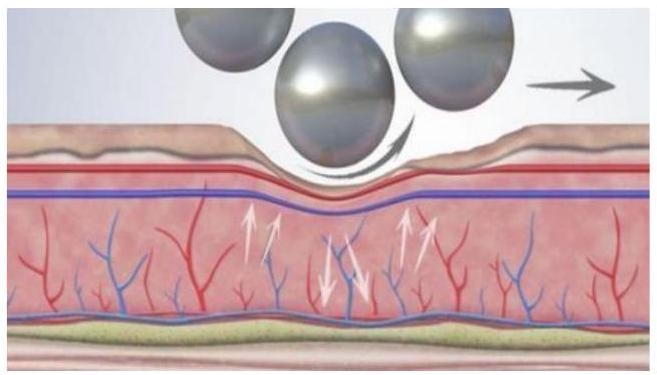
\includegraphics[max width=\textwidth, alt={}, center]{31d8a32b-88de-483b-82f7-0d2b231ca911-04_375_657_2435_191}

\begin{figure}[H]
\begin{center}
  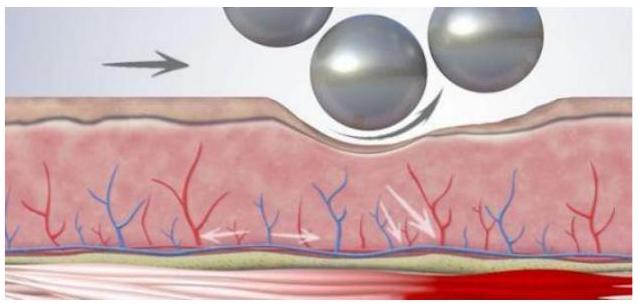
\includegraphics[alt={},max width=\textwidth]{31d8a32b-88de-483b-82f7-0d2b231ca911-04_305_638_1155_1014}
\captionsetup{labelformat=empty}
\caption{Azione muscolare}
\end{center}
\end{figure}

Tonifica i muscoli e rassoda i tessuti.

\begin{figure}[H]
\begin{center}
  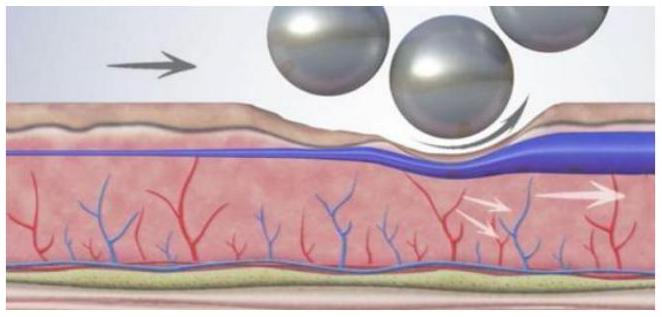
\includegraphics[alt={},max width=\textwidth]{31d8a32b-88de-483b-82f7-0d2b231ca911-04_317_662_1790_1027}
\captionsetup{labelformat=empty}
\caption{Azione di drenaggio}
\end{center}
\end{figure}

Elimina le tossine e favorisce il drenaggio linfatico.

Effetto vascolare

Migliora la circolazione sanguigna e nutre i tessuti.

\newpage

\section{Caratteristiche:}
\begin{enumerate}
  \item C'è una maniglia grande e una maniglia piccola.
  \item Le sfere del manubrio sono sostituibili. Tutte le maniglie includono un set di sfere metalliche e un altro di Silicone. (Nota: non sono sostituibili sul mercato.)
  \item 10 velocità regolabili e ogni maniglia ha una luce:
  \begin{itemize}
  	\item  luce rossa
  	\item luce blu 
  	\item luce verde
  \end{itemize}
  \item Ci sono tre modalità di illuminazione opzionali per ogni colore, Tutte le ruote della maniglia consentono il movimento bidirezionale e può memorizzare 5 set di parametri operazioni.
  \item Custodia stampata a iniezione, touchscreen da 5,6" pollici, flight case e imballaggio di alta qualità.
\end{enumerate}





\section{Parte dell'applicazione}
\begin{center}
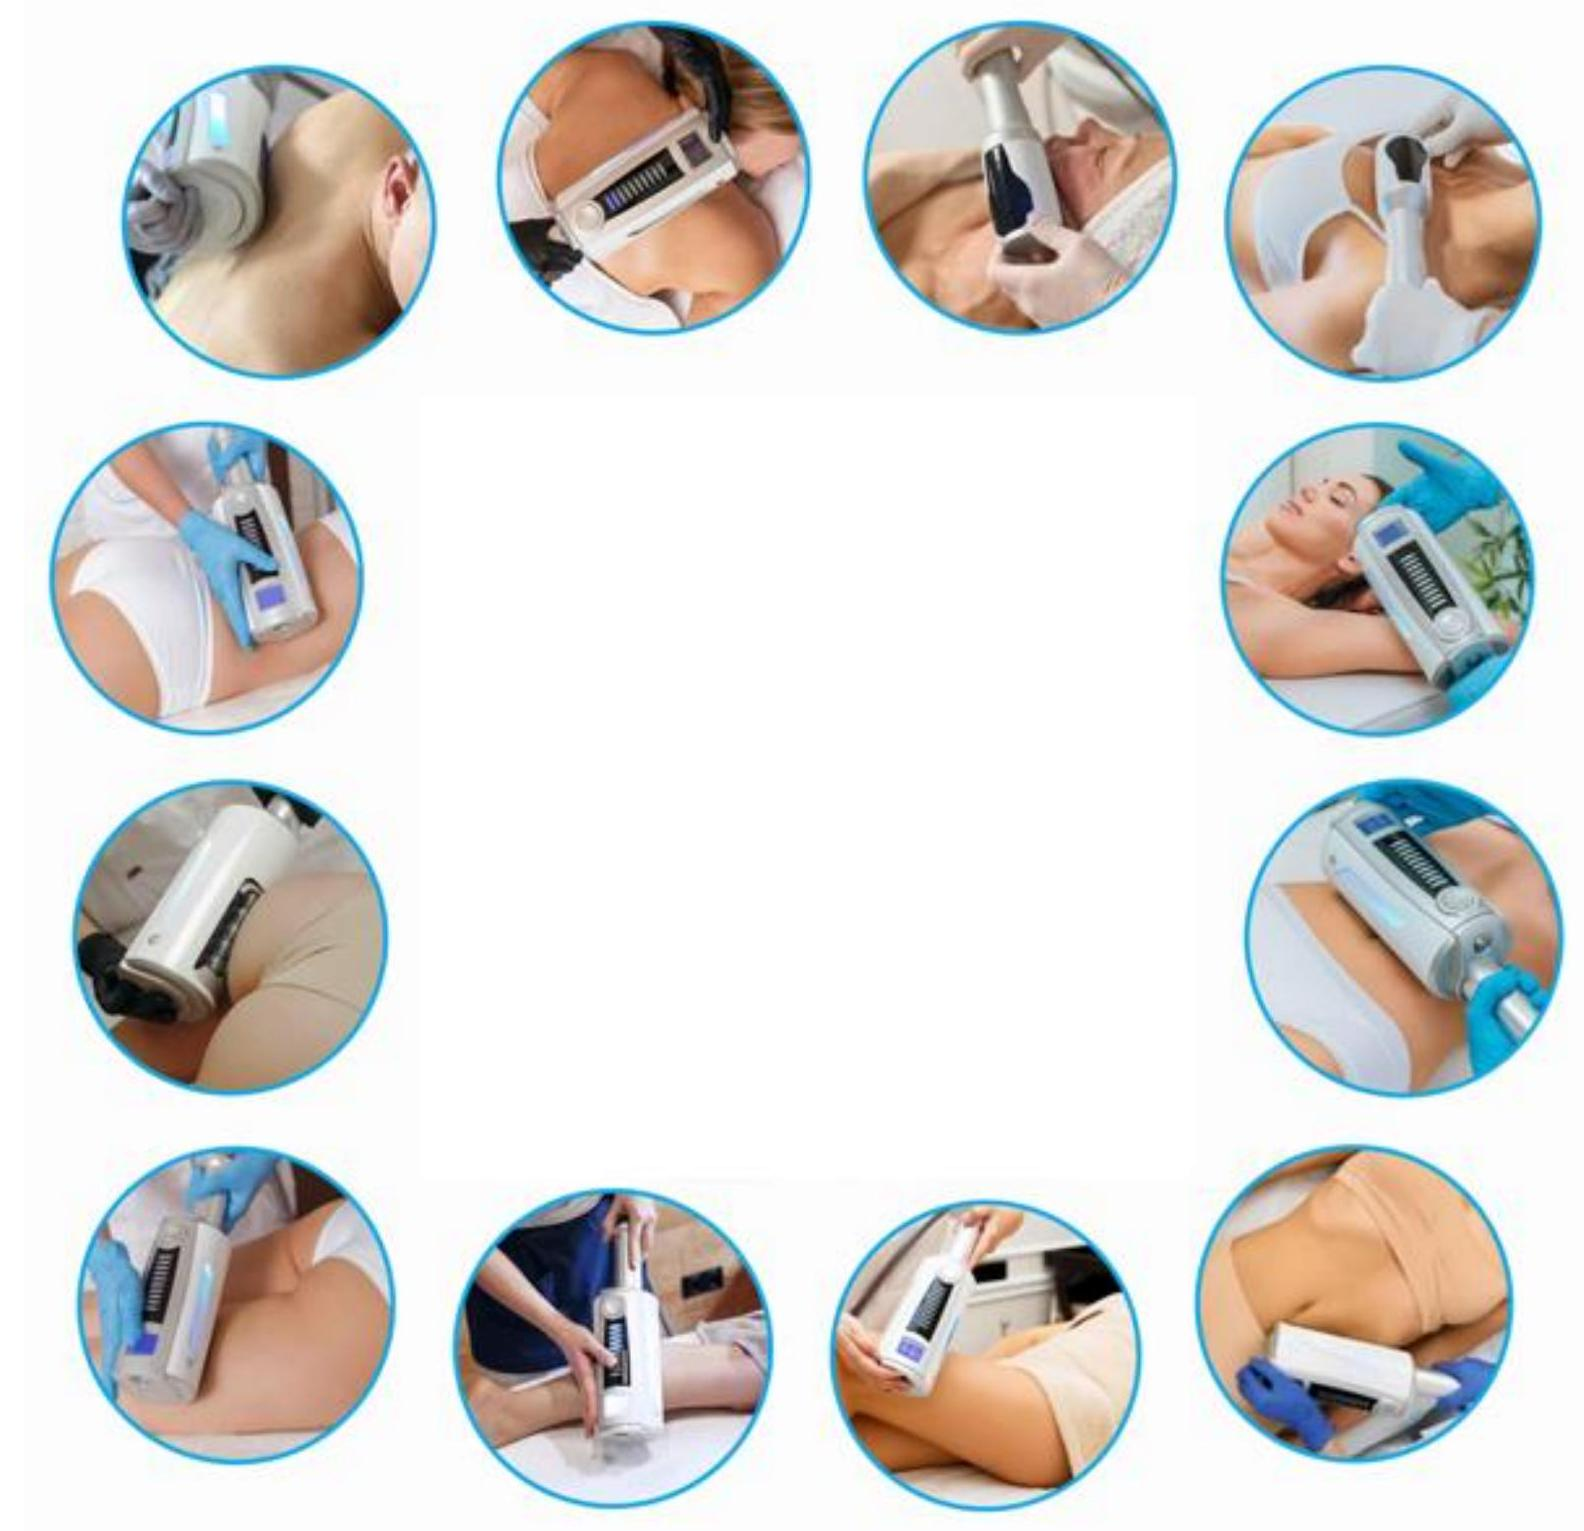
\includegraphics[max width=\textwidth, alt={}]{31d8a32b-88de-483b-82f7-0d2b231ca911-06_1531_1584_338_164}
\end{center}

\section{Istruzioni per lo strumento}
A. Installazione: allineare la maniglia con l'apposita presa sul retro del dispositivo e posizionarlo sullo scaffale; inserire il cavo di alimentazione nella presa sul retro del dispositivo, accendere il dispositivo e accendere l'interruttore di alimentazione, quindi premere il pulsante di accensione per avviare il dispositivo.\\
B. Manico piccolo: da utilizzare su viso, collo e spalle.\\
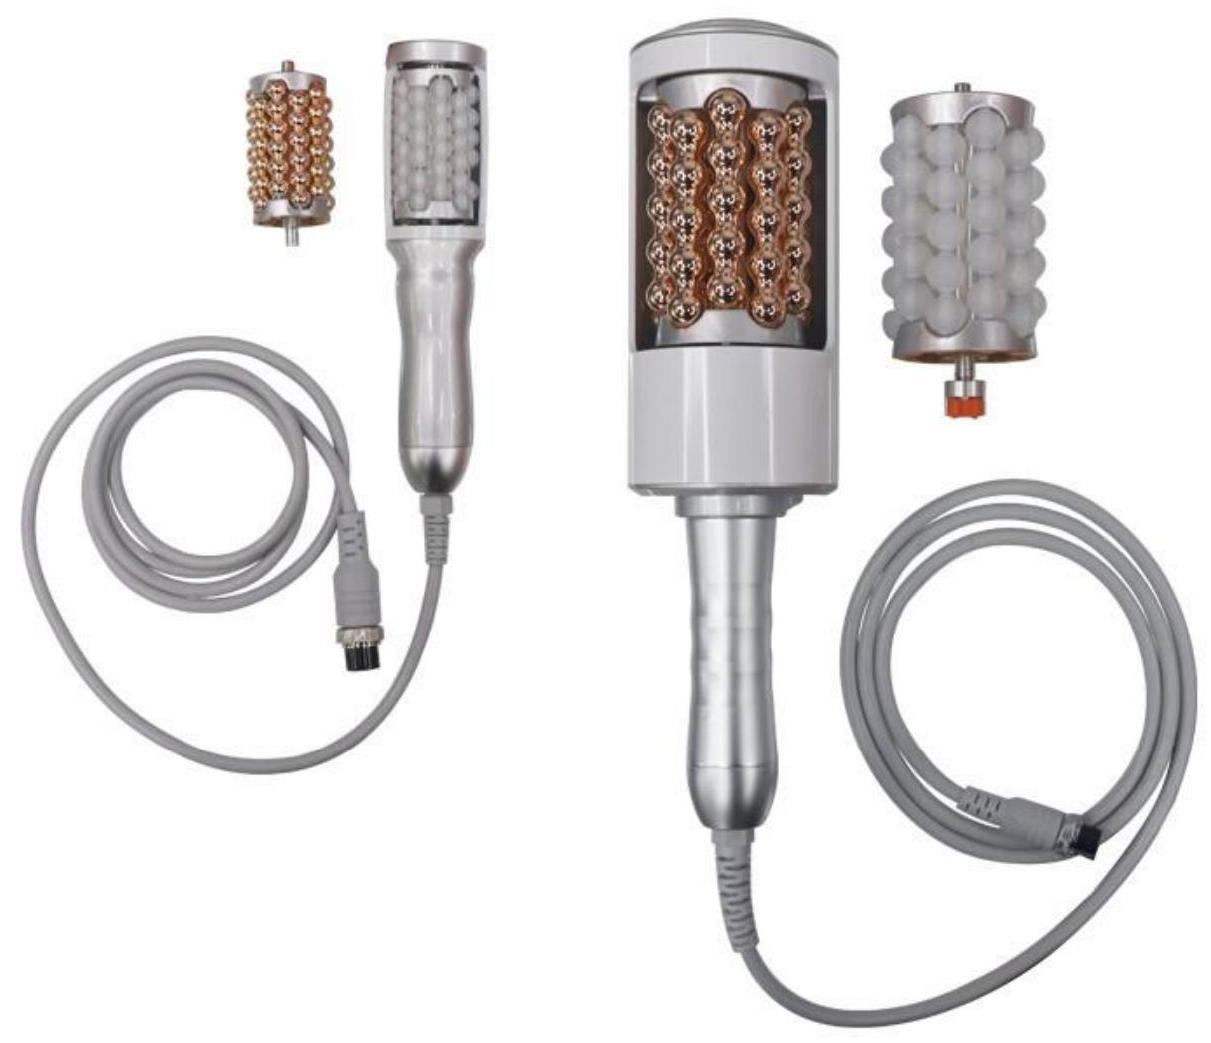
\includegraphics[max width=\textwidth, alt={}, center]{31d8a32b-88de-483b-82f7-0d2b231ca911-07_1043_1211_648_395}\\
C.Manico grande: da utilizzare sul corpo.\\
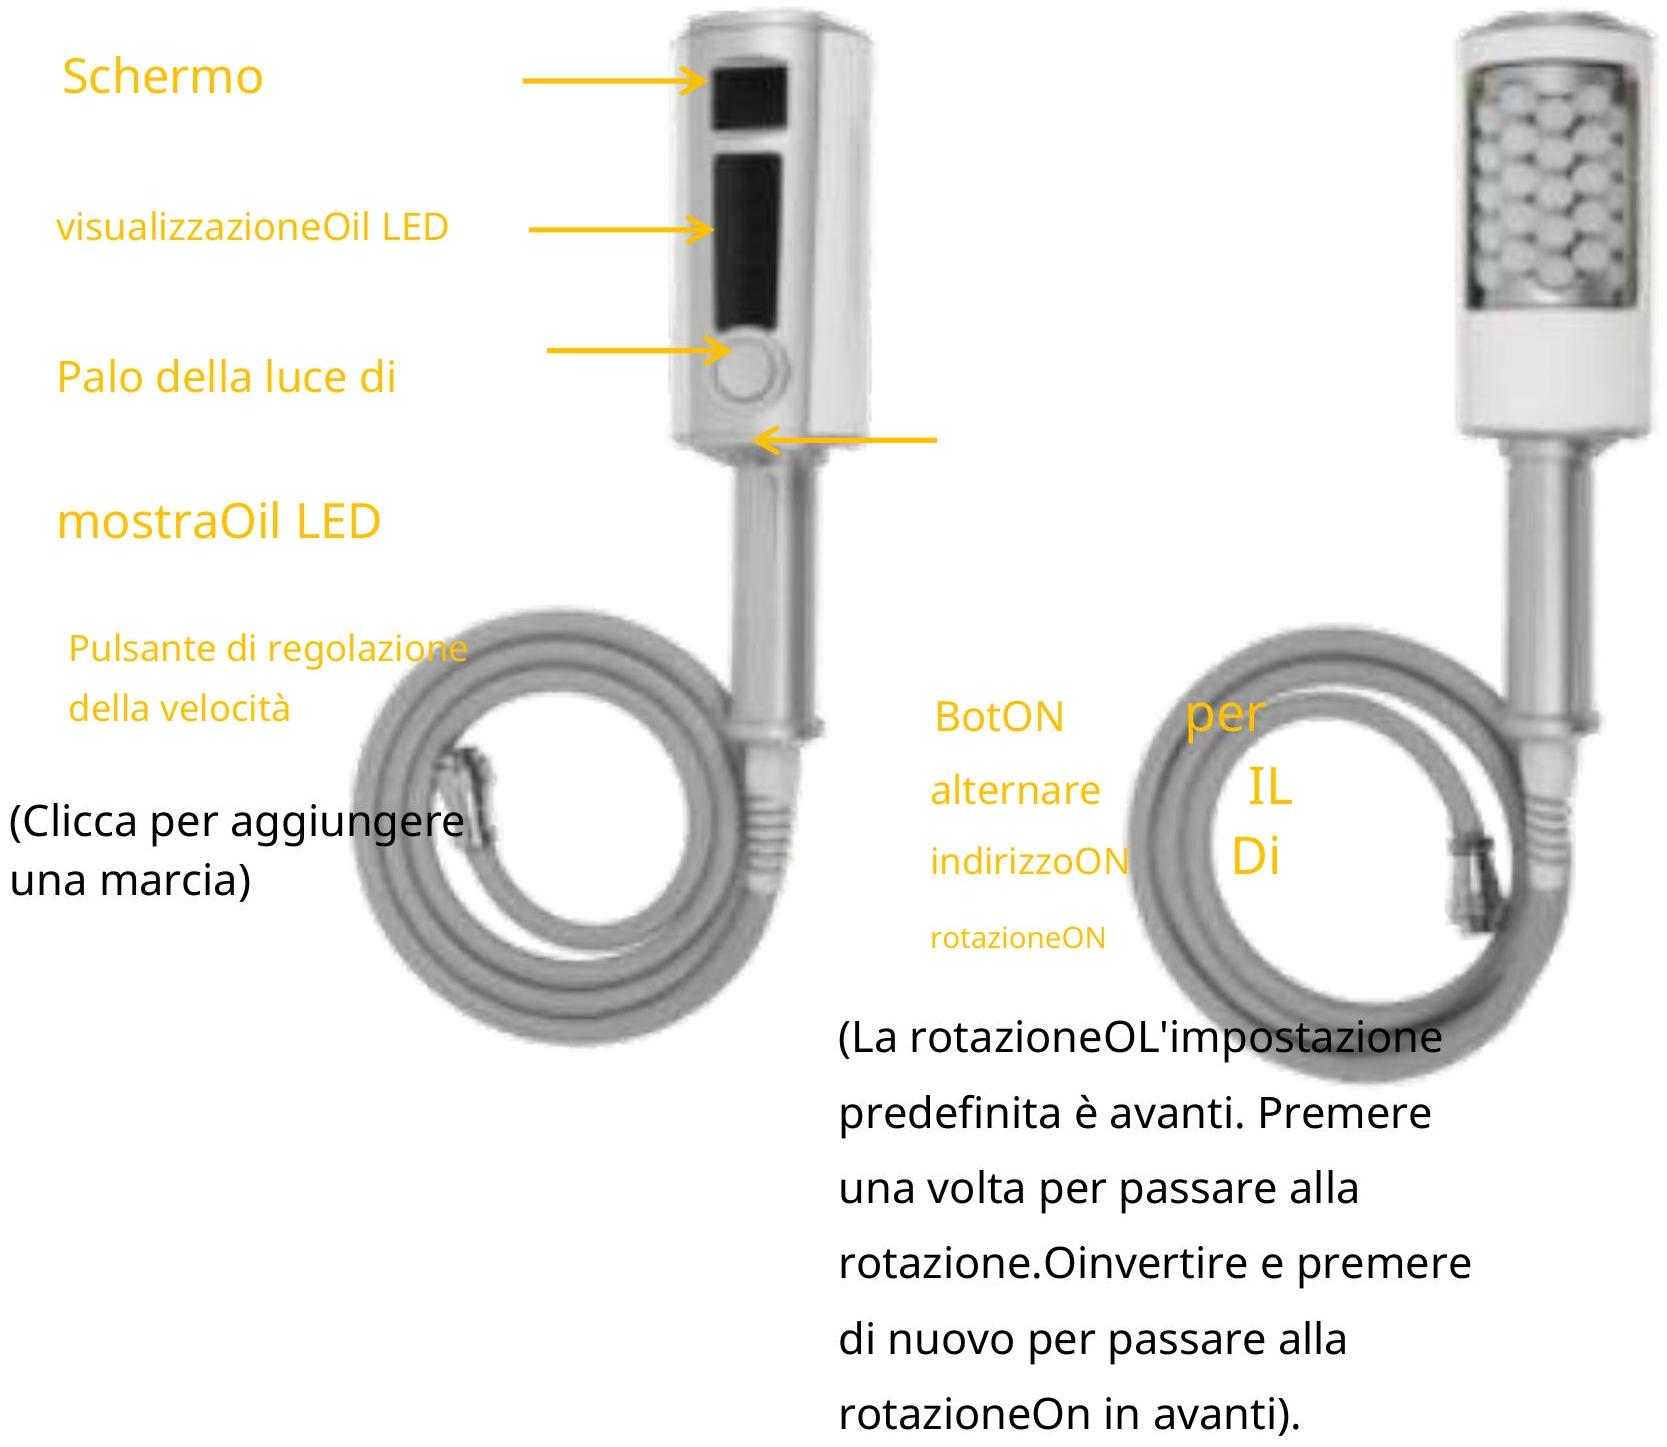
\includegraphics[max width=\textwidth, alt={}, center]{31d8a32b-88de-483b-82f7-0d2b231ca911-08_1447_1667_411_207}

\begin{figure}[H]
\begin{center}
  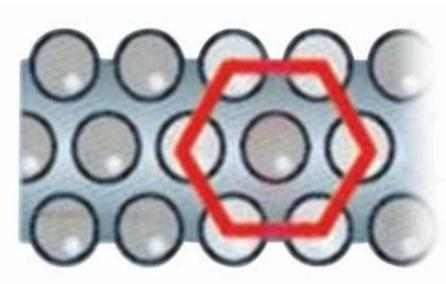
\includegraphics[alt={},max width=\textwidth]{31d8a32b-88de-483b-82f7-0d2b231ca911-08_284_446_2101_157}
\captionsetup{labelformat=empty}
\caption{Fornitura di sfere a forma di nido d'ape}
\end{center}
\end{figure}

\begin{figure}[H]
\begin{center}
  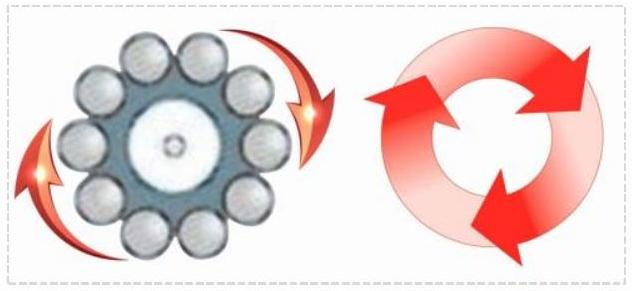
\includegraphics[alt={},max width=\textwidth]{31d8a32b-88de-483b-82f7-0d2b231ca911-08_291_632_2101_641}
\captionsetup{labelformat=empty}
\caption{Rotazione in senso orario\\
(Abbreviazione: rotazione) in senso orario)}
\end{center}
\end{figure}

\begin{figure}[H]
\begin{center}
  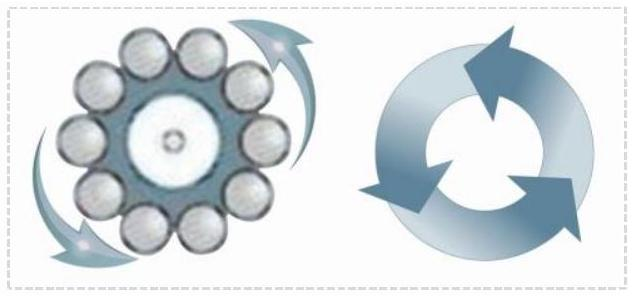
\includegraphics[alt={},max width=\textwidth]{31d8a32b-88de-483b-82f7-0d2b231ca911-08_296_632_2101_1315}
\captionsetup{labelformat=empty}
\caption{Girare nella direzione\\
in senso antiorario}
\end{center}
\end{figure}

(Abbreviazione: inverso)\\
D. La sostituzione e l'installazione del rullo integrato nella maniglia sono illustrate nella figura seguente:

\begin{figure}[H]
\begin{center}
  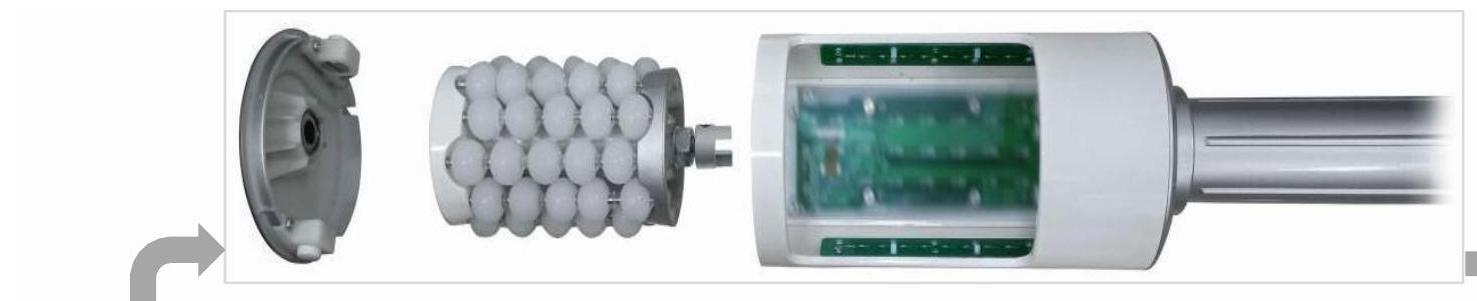
\includegraphics[alt={},max width=\textwidth]{31d8a32b-88de-483b-82f7-0d2b231ca911-09_301_1477_424_182}
\captionsetup{labelformat=empty}
\caption{2. Rimuovere il corpo del rullo a sfera in silicone}
\end{center}
\end{figure}

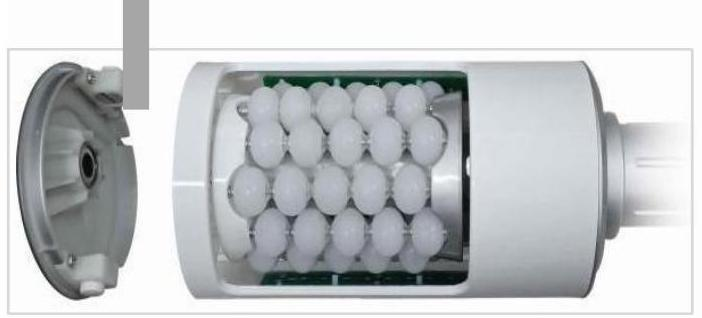
\includegraphics[max width=\textwidth, alt={}, center]{31d8a32b-88de-483b-82f7-0d2b231ca911-09_318_702_781_189}\\
(1) Premere e tenere premuti contemporaneamente i pulsanti su entrambi i lati.

\begin{figure}[H]
\begin{center}
  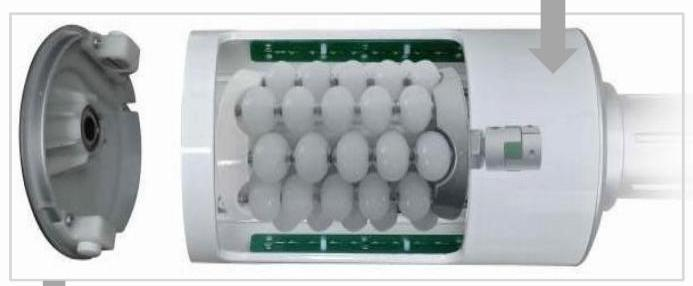
\includegraphics[alt={},max width=\textwidth]{31d8a32b-88de-483b-82f7-0d2b231ca911-09_286_693_804_1160}
\captionsetup{labelformat=empty}
\caption{(3) Sostituire e installare un nuovo}
\end{center}
\end{figure}

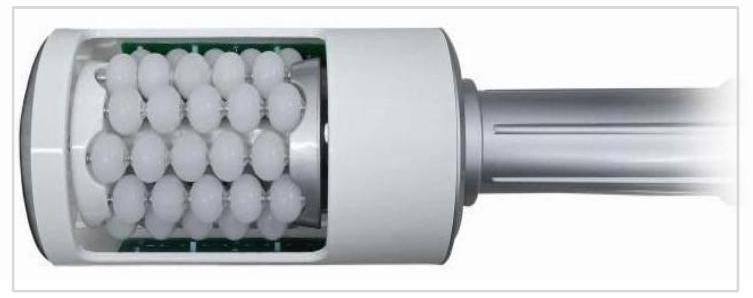
\includegraphics[max width=\textwidth, alt={}, center]{31d8a32b-88de-483b-82f7-0d2b231ca911-09_298_753_1199_648}\\
(4) Allinea il corpo dell'asse y

Installare il coperchio nello slot.

\section{Introduzione all'interfaccia}
A. Verificare che il collegamento dello strumento sia corretto. Collegare lo strumento all'alimentazione e accenderlo. Premere il pulsante di accensione e il dispositivo si accenderà immediatamente. Apparirà l'interfaccia di avvio.

\begin{figure}[H]
\begin{center}
  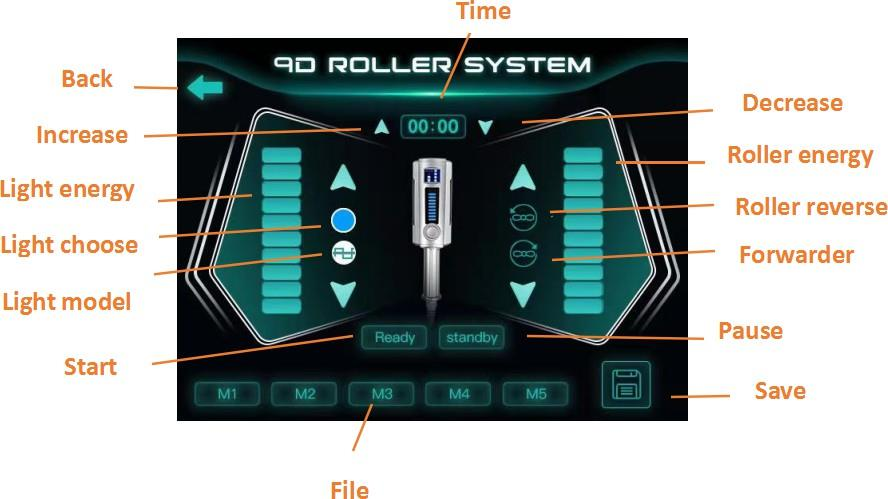
\includegraphics[alt={},max width=\textwidth]{31d8a32b-88de-483b-82f7-0d2b231ca911-10_968_1876_1251_100}
\captionsetup{labelformat=empty}
\caption{IO}
\end{center}
\end{figure}

\begin{figure}[H]
	\centering
	\includegraphics[width=\linewidth]{"images/Schermata del 2026-03-09 13-24-29"}
%	\caption{}
	\label{fig:schermata-del-2026-03-09-13-24-29}
\end{figure}


\section{Cos'è una macchina a rulli a sfere interne?}
Il rullo a sfere interno è uno strumento all'avanguardia per il body shaping, Riconosciuto a livello mondiale. Utilizza l'innovativa microvibrazione a compressione per migliorare drenaggio linfatico, aumento della circolazione sanguigna, miglioramento della cellulite, riduzione della cellulite, inversione della cellulite Combatte i segni dell'invecchiamento, condiziona i muscoli e disintossica. Può essere utilizzato su Viso e corpo. Le zone più richieste per il trattamento sono cosce, glutei e... parte superiore delle braccia.

\section{La terapia microvibrazionale compressiva è sicura?}
La terapia compressiva microvibrazionale è un trattamento non invasivo e sicuro al 100\%. e non ha effetti collaterali.

\section{Quanto dura un singolo trattamento?}
È adatto a qualsiasi parte del corpo o del viso, ma a seconda delle dimensioni del Il tempo di trattamento per la zona varierà da un minimo di circa 45 minuti ad un massimo di 1 ora e 30 minuti.

\section{Sentirai dolore durante il trattamento?}
No, è un trattamento molto piacevole. La maggior parte dei clienti afferma di sentirsi Simile a un massaggio dei tessuti profondi. L'intensità/livello di stress aumenta gradualmente. ad ogni seduta e può essere regolato in base alla tolleranza desiderata. Non ha effetti collaterali. effetti collaterali e può tornare alla vita normale subito dopo il trattamento.

\section{Con quale frequenza può essere eseguito il trattamento?}
In genere si consiglia di farlo due o tre volte a settimana. Tuttavia, il tempo Il tempo minimo tra una sessione e l'altra è di 48 ore.

\begin{table}[H]
\begin{center}
\captionsetup{labelformat=empty}
\caption{Parametri del prodotto}
\begin{tabularx}{\textwidth}{|X|X|}
\hline
Nome del prodotto & Macchina a rulli a sfere interne \\
\hline
Schermo tattile & Ampio schermo LCD da 5,6 pollici \\
\hline
Grande velocità della maniglia & 450 giri al minuto \\
\hline
Piccola velocità della maniglia & 410 giri al minuto \\
\hline
Frequenza di uscita & $40-254 \mathrm{~Hz}$ \\
\hline
Tensione di ingresso & CA $110 \mathrm{~V} / 220 \mathrm{~V}$ \\
\hline
Potenza di uscita & $100-1000 \mathrm{~W}$ \\
\hline
Fusibile & 5A \\
\hline
mango grande & 50 palline in silicone (per la cura del corpo) \\
\hline
piccola maniglia & 60 palline in silicone (per la cura del viso e del collo) \\
\hline
Temperatura ambiente & $5^{\circ} \mathrm{C} \sim+40^{\circ} \mathrm{C}$ \\
\hline
\end{tabularx}
\end{center}
\end{table}

\documentclass[10pt]{article}
\usepackage[italian]{babel}
\usepackage[utf8]{inputenc}
\usepackage[T1]{fontenc}
\usepackage{amsmath}
\usepackage{amsfonts}
\usepackage{amssymb}
\usepackage[version=4]{mhchem}
\usepackage{stmaryrd}

\begin{document}
\section{CONSENSO INFORMATO}
\section{Trattamento estetico "RollerShape+"}
\section{DATI CLIENTE}
Nome e Cognome: $\_\_\_\_$\\
Data di nascita: $\_\_\_\_$\\
Telefono: $\_\_\_\_$

\section{DATI OPERATORE / CENTRO}
Nome centro: $\_\_\_\_$\\
Operatore: $\_\_\_\_$

\section{DESCRIZIONE DEL TRATTAMENTO}
Il trattamento RollerShape+ utilizza una tecnologia a rulli compressivi per stimolare il microcircolo, favorire il drenaggio dei liquidi, migliorare la tonicità dei tessuti e contrastare gli inestetismi della cellulite.

\section{POSSIBILI EFFETTI}
Lieve arrossamento temporaneo, sensazione di pressione o calore, lieve sensibilità nella zona trattata.

\section{CONTROINDICAZIONI}
Gravidanza, fragilità capillare importante, problemi circolatori severi, patologie oncologiche in corso, infezioni o infiammazioni nella zona trattata, presenza di ematomi o lesioni cutanee.

\section{DICHIARAZIONI DEL CLIENTE}
Dichiaro di aver ricevuto spiegazioni chiare, di essere a conoscenza che si tratta di trattamento estetico e non medico, e di autorizzare l'esecuzione del trattamento.

\section{PRIVACY}
I dati saranno trattati nel rispetto del Regolamento UE 2016/679 (GDPR).\\
Firma Cliente: $\_\_\_\_$\\
Firma Operatore: $\_\_\_\_$\\
Data: $\_\_\_\_$ 1 $\_\_\_\_$ $/$ $\_\_\_\_$


\end{document}

% --- INIZIO INFORMATIVA PRIVACY ---
\newpage

\section{INFORMATIVA PRIVACY}
\begin{center}
	(ai sensi dell'art. 13 del Regolamento UE 2016/679)
\end{center}

La presente informativa è resa ai sensi del Regolamento Generale sulla Protezione dei Dati (GDPR) e riguarda il trattamento dei dati personali dei clienti che si sottopongono a trattamenti e tecnologie estetiche.

\subsection*{Titolare del trattamento}

Il Titolare del trattamento è:

\begin{itemize}
	\item Denominazione centro estetico: \underline{\hspace{5cm}}
	\item Sede legale: \underline{\hspace{7cm}}
	\item P. IVA / C.F.: \underline{\hspace{6cm}}
	\item Contatti (telefono/email): \underline{\hspace{5cm}}
\end{itemize}

\subsection*{Tipologia di dati trattati}

Il Titolare può raccogliere e trattare le seguenti categorie di dati:

\begin{itemize}
	\item Dati anagrafici (nome, cognome, data di nascita)
	\item Dati di contatto (telefono, e-mail)
	\item Dati fiscali per eventuale fatturazione
	\item Dati particolari relativi allo stato di salute (allergie, patologie, gravidanza, terapie in corso) necessari per valutare l'idoneità ai trattamenti estetici
	\item Eventuali immagini fotografiche prima/dopo trattamento (previo consenso specifico)
\end{itemize}

\subsection*{Finalità del trattamento}

I dati personali sono trattati per le seguenti finalità:

\begin{enumerate}
	\item Esecuzione di trattamenti estetici e utilizzo di tecnologie professionali (laser, radiofrequenza, ultrasuoni, pressoterapia, ecc.)
	\item Valutazione dell'idoneità al trattamento
	\item Adempimenti amministrativi, contabili e fiscali
	\item Gestione degli appuntamenti
	\item Eventuale invio di comunicazioni promozionali (solo previo consenso separato)
	\item Eventuale utilizzo di immagini per finalità informative o promozionali (solo previo consenso separato)
\end{enumerate}

\subsection*{Base giuridica del trattamento}

Il trattamento dei dati si fonda su:

\begin{itemize}
	\item Esecuzione del contratto/prestazione richiesta
	\item Adempimento di obblighi di legge
	\item Consenso esplicito dell'interessato per il trattamento di dati particolari (sanitari)
	\item Consenso separato per marketing e utilizzo immagini
\end{itemize}

\subsection*{Modalità di trattamento}

Il trattamento dei dati avviene mediante strumenti cartacei e/o informatici, nel rispetto dei principi di correttezza, liceità, trasparenza e tutela della riservatezza.

Sono adottate adeguate misure di sicurezza per prevenire accessi non autorizzati, perdita o diffusione dei dati.

\subsection*{Conservazione dei dati}

I dati personali saranno conservati:

\begin{itemize}
	\item Per il tempo necessario all'erogazione del servizio
	\item Per il periodo previsto dalla normativa fiscale e civilistica
	\item Fino a revoca del consenso per finalità di marketing o utilizzo immagini
\end{itemize}

\subsection*{Comunicazione dei dati}

I dati potranno essere comunicati a:

\begin{itemize}
	\item Consulenti fiscali e amministrativi
	\item Software gestionali utilizzati per la gestione clienti
	\item Autorità competenti, ove previsto dalla legge
\end{itemize}

I dati non saranno diffusi senza consenso.

\subsection*{Diritti dell'interessato}

L'interessato può esercitare in qualsiasi momento i seguenti diritti:

\begin{itemize}
	\item Accesso ai propri dati
	\item Rettifica o aggiornamento
	\item Cancellazione (diritto all'oblio)
	\item Limitazione del trattamento
	\item Opposizione al trattamento
	\item Revoca del consenso
	\item Reclamo all'Autorità Garante per la Protezione dei Dati Personali
\end{itemize}

Le richieste possono essere inviate ai recapiti del Titolare sopra indicati.

\subsection*{Natura del conferimento dei dati}

Il conferimento dei dati è necessario per l'erogazione dei trattamenti estetici.
Il mancato conferimento può comportare l'impossibilità di eseguire il servizio.

\subsection*{CONSENSO}

Il/La sottoscritto/a dichiara di aver ricevuto e compreso la presente informativa.

\vspace{0.8cm}

Data: \underline{\hspace{5cm}} 

\vspace{15pt}
Firma: \underline{\hspace{6cm}}

\vspace{1cm}

$\square$ Acconsento al trattamento dei dati particolari (sanitari)

\vspace{0.3cm}
$\square$ Acconsento all'utilizzo delle immagini per finalità promozionali

\vspace{0.3cm}
$\square$ Acconsento a ricevere comunicazioni promozionali

% --- FINE INFORMATIVA PRIVACY ---

\newpage


\begin{figure}[H]
	\centering
	\includegraphics[width=0.7\paperwidth,height=\paperheight, keepaspectratio]{"../cose da aggiungere/privacy_conformita/dichiarazione_conformita"}
\end{figure}


\end{document}